


\documentclass[landscape,color=UCLdarkred,margin=3cm]{uclposter}

\usepackage[T1]{fontenc}
\usepackage{lmodern,textcomp}
\usepackage{amsmath,amssymb}
\usepackage{amsthm}
\usepackage{xcolor}
\usepackage{eso-pic}
\usepackage{authblk}
\usepackage{tikz}
\usepackage{environ}
\usepackage{ulgothic}
\usepackage{graphicx}
\usepackage{float}
\usepackage{physics}

\title{Scalable Quantum Simulation of Molecular Energies}

\author[1 *]{Shuhao Yang}
\author[1,2]{James Mills}
\author[1,2]{Shanice St John}
\affil[1]{Department of LaTeX Studies, UCL}
\affil[2]{TikZ, UCL}
\affil[*]{a.example@ucl.ac.uk}

\begin{document}

\maketitle

\begin{multicols}{3}

\section*{Introduction}
A poster class for \LaTeX that attempts to follow the UCL Corporate Identity.
This package is unofficial and is not supported by UCL.

Currently only compilation with XeLaTeX is supported.

\section*{Installation and usage}

Copy the `uclposter.sty` file to the directory containing the poster LaTeX file.
No additional files are needed (the banner/logo is included entirely as vector drawing code).

\section*{Highlight boxes}

\begin{highlightbox}
	The \textbackslash highlightbox command inserts a coloured box, the default colour is a lighter version of the banner colour.
\end{highlightbox}

\begin{highlightbox}[UCLdarkblue!20!white]
	The colour of a \textbackslash highlightbox can also be changed.
\end{highlightbox}

\begin{highlightbox}[UCLdarkblue!20!white]
	Qubit
\end{highlightbox}

\begin{highlightbox}[UCLdarkblue!20!white]
	Qubit
\end{highlightbox}

\begin{highlightbox}[UCLdarkblue!20!white]
	Qubit
\end{highlightbox}

\columnbreak

\section*{Techniques in Paper}



\begin{figure}[H]
  \begin{center}
  \begin{minipage}[c]{16em}
    
    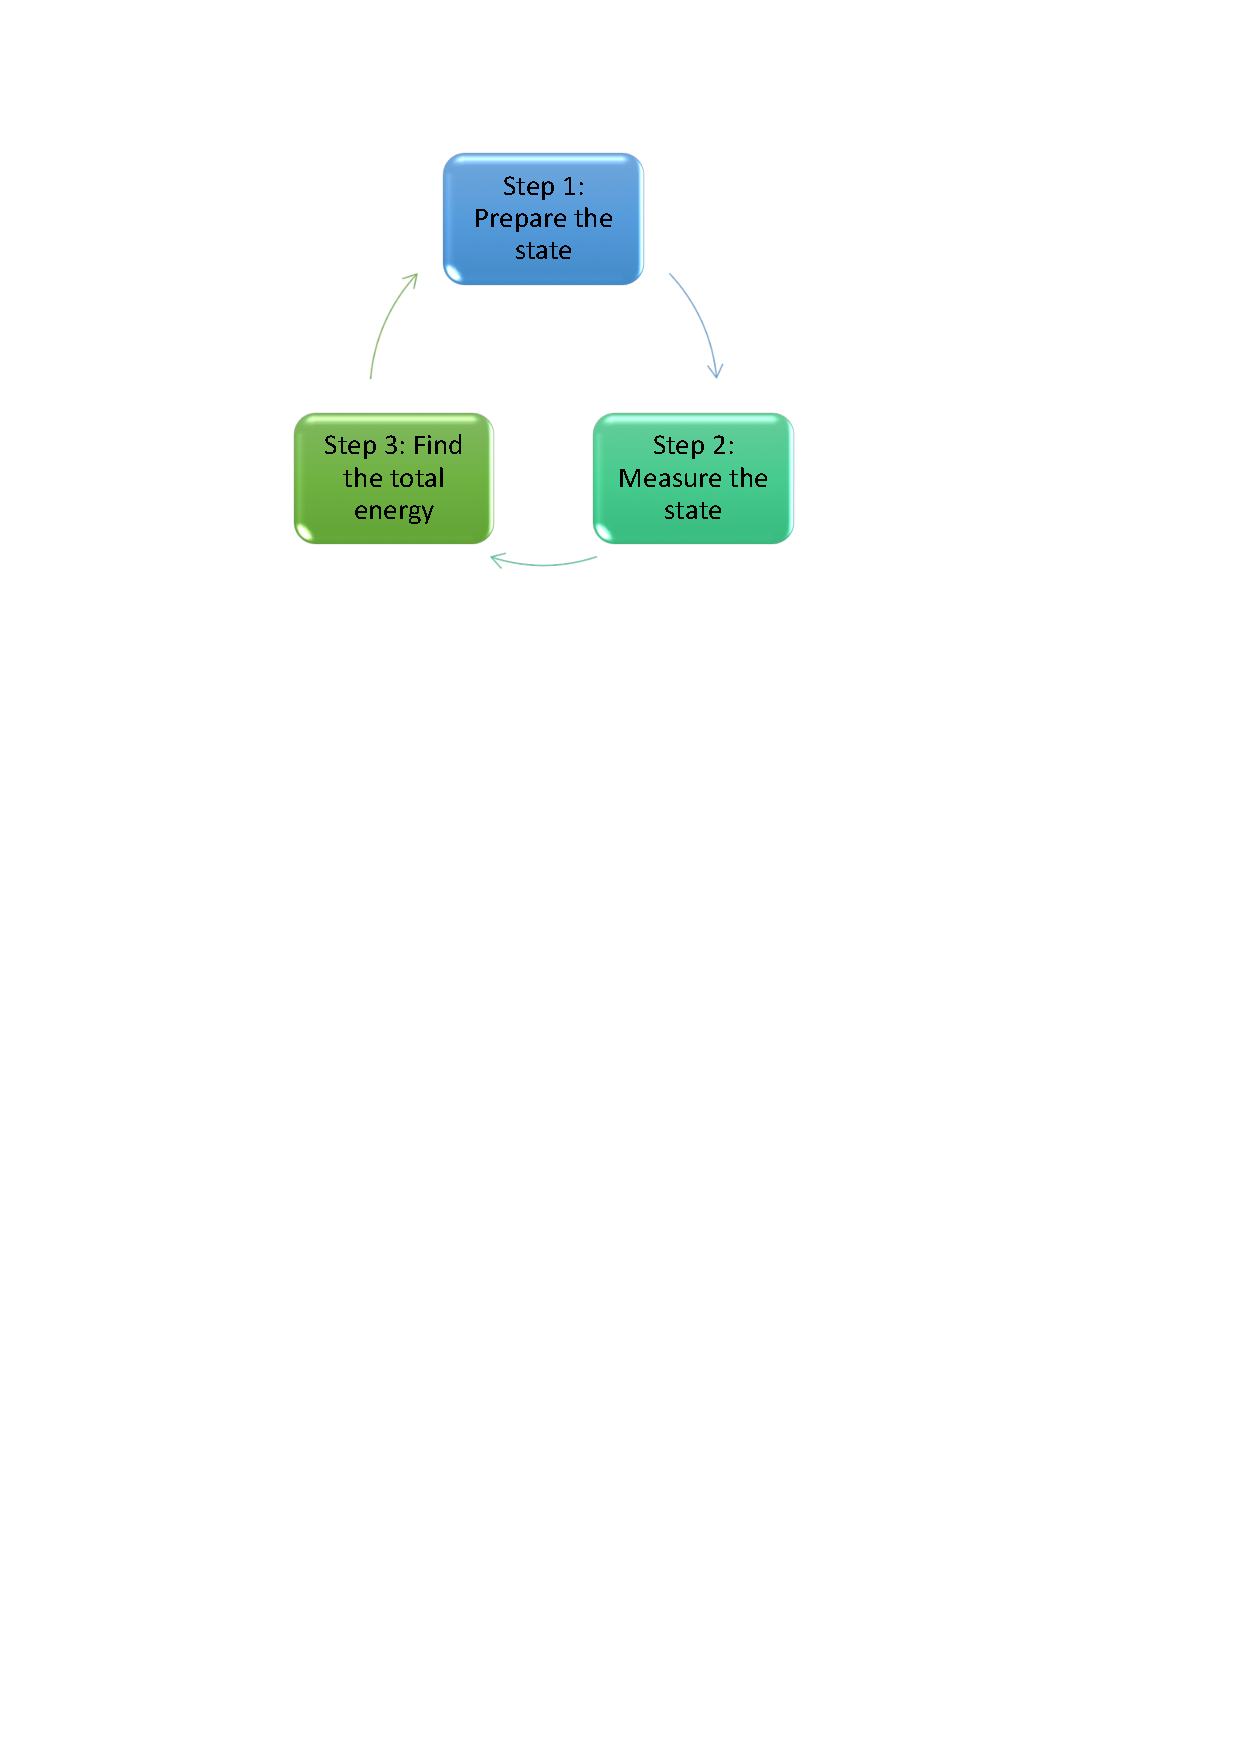
\includegraphics[width=16em]{VQEdiagram.pdf}
    \caption{VQE}
  \end{minipage}
  \qquad
  \begin{minipage}[c]{18em}
    \centering
    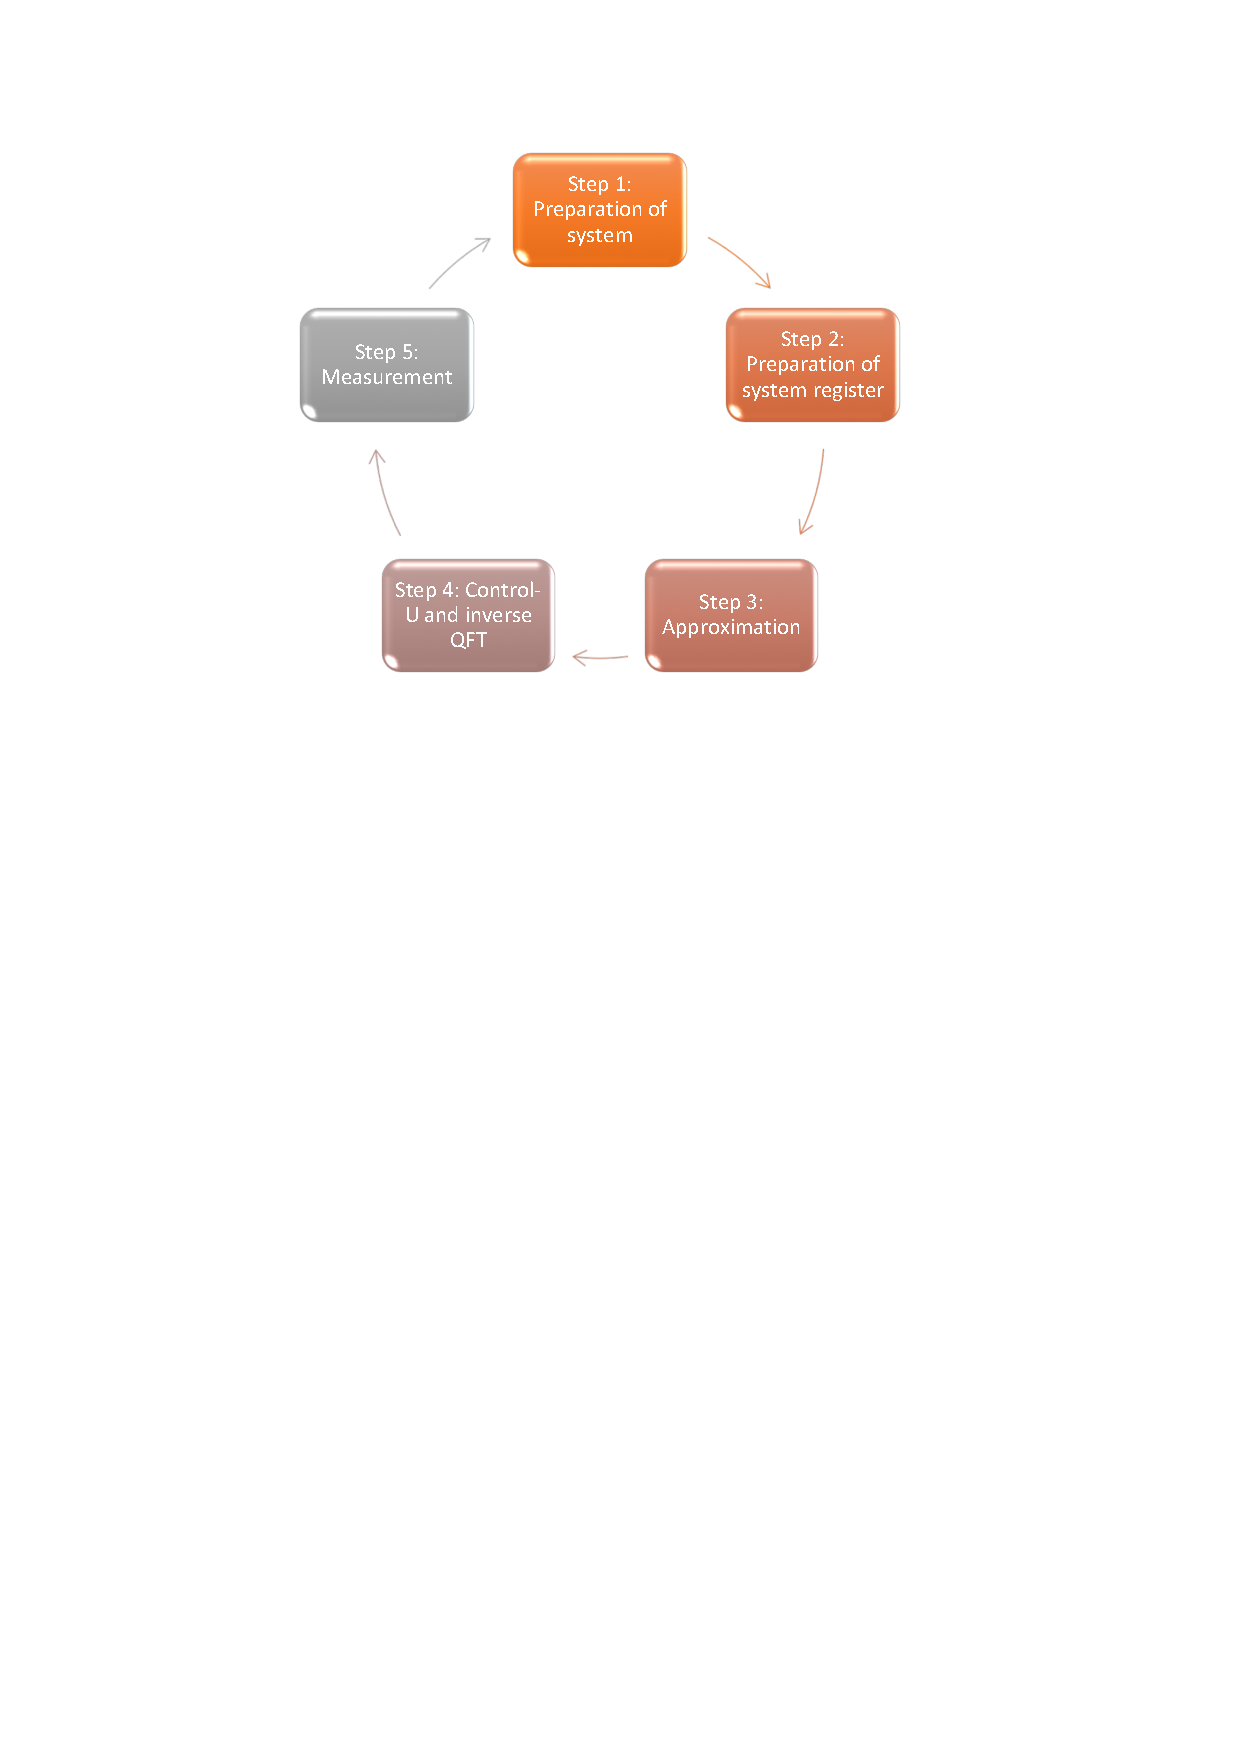
\includegraphics[width=18em]{PEA.pdf}
    \caption{PEA}
  \end{minipage}
  \end{center}

   
\end{figure}

\begin{tikzpicture}
	\foreach \x[count=\xi] in {UCLlightpurple, UCLdarkpurple, UCLpurple, UCLblueceleste, UCLlightblue, UCLskyblue, UCLbrightblue, UCLnavyblue, UCLdarkblue, UCLdarkgreen, UCLmidgreen, UCLbrightgreen, UCLlightgreen, UCLstone, UCLdarkgrey, UCLdarkbrown, UCLdarkred, UCLburgundy, UCLpink, UCLrichred, UCLmidred, UCLorange, UCLyellow, UCLwhite, UCLblack}
	{
	\fill[fill=\x] (0,-\xi) rectangle +(0.9,0.9) node[anchor=north west, inner sep=3pt] {\x};
	}
\end{tikzpicture}

\columnbreak

\section*{Conclusion and Outlook}

\begin{highlightbox}[UCLdarkblue!20!white]
	The colour of a \textbackslash highlightbox can also be changed.
\end{highlightbox}



\end{multicols}
	
\end{document}
